\documentclass[11pt,a4paper]{article}
\usepackage[utf8]{inputenc}
\usepackage[T1]{fontenc}
\usepackage{lmodern}
\usepackage[top=0.85in, bottom=0.85in, left=0.8in, right=0.8in]{geometry}
\usepackage{amsmath,amsfonts,amssymb}
\usepackage{graphicx}
\usepackage{hyperref}
\usepackage{booktabs}
\usepackage{array}
\usepackage{listings}
\usepackage{xcolor}
\usepackage{float}
\usepackage{caption}
\usepackage{subcaption}
\usepackage{titlesec}
\usepackage{enumitem}
\usepackage[most]{tcolorbox}
\usepackage{microtype}
\usepackage{tikz}
\usetikzlibrary{shapes.geometric, arrows.meta, positioning, fit, backgrounds, calc}

% ---------- Colors ----------
\definecolor{primarycolor}{RGB}{31, 78, 121}
\definecolor{secondarycolor}{RGB}{0, 102, 204}
\definecolor{codegreen}{rgb}{0,0.6,0}
\definecolor{codegray}{rgb}{0.5,0.5,0.5}
\definecolor{codepurple}{rgb}{0.58,0,0.82}
\definecolor{backcolour}{rgb}{0.96,0.96,0.96}
\definecolor{boxbg}{RGB}{238, 244, 251}

% ---------- Code style ----------
\lstdefinestyle{mystyle}{
    backgroundcolor=\color{backcolour},
    commentstyle=\color{codegreen},
    keywordstyle=\color{primarycolor}\bfseries,
    numberstyle=\tiny\color{codegray},
    stringstyle=\color{codepurple},
    basicstyle=\ttfamily\footnotesize,
    breakatwhitespace=false,
    breaklines=true,
    captionpos=b,
    keepspaces=true,
    numbers=left,
    numbersep=8pt,
    showspaces=false,
    showstringspaces=false,
    showtabs=false,
    tabsize=2,
    frame=single,
    rulecolor=\color{codegray!50}
}
\lstset{style=mystyle}

% ---------- Hyperref ----------
\hypersetup{
    colorlinks=true,
    linkcolor=primarycolor,
    urlcolor=secondarycolor,
    pdftitle={Lab Assignment: Docker Containerization Report},
    pdfauthor={Sunil Kumar}
}

% ---------- Sections ----------
\titleformat{\section}{\large\bfseries\color{primarycolor}}{\thesection.}{0.5em}{}
\titleformat{\subsection}{\normalsize\bfseries\color{secondarycolor}}{\thesubsection}{0.5em}{}
\titlespacing*{\section}{0pt}{10pt}{4pt}
\titlespacing*{\subsection}{0pt}{8pt}{3pt}

\setlength{\parskip}{4pt}
\setlength{\parindent}{0pt}

\raggedbottom
\captionsetup{font=small, labelfont=bf, skip=4pt}
\pagestyle{plain}

\begin{document}

% =========================================================
% TITLE BLOCK
% =========================================================
\begin{center}
    {\LARGE \bfseries \color{primarycolor} Containerization of Proximity Search API}\\[0.2cm]
    {\large \bfseries Full-Stack Multi-Service Orchestration via Docker and Docker Compose}\\[0.3cm]
    {\large \textbf{Name:} Sunil Kumar \quad $|$ \quad \textbf{ID:} 12342170}
\end{center}

\begin{tcolorbox}[colback=boxbg, colframe=primarycolor, boxrule=0.8pt, arc=3pt,
                  title={\bfseries Project \& Environment Overview}, fonttitle=\small, left=6pt, right=6pt, top=3pt, bottom=3pt]
\small
\begin{tabular}{@{}p{0.28\linewidth}p{0.68\linewidth}@{}}
\textbf{Assignment:} & Docker Containerization of Proximity Search API \\[2pt]
\textbf{Host Machine:} & Personal Workstation (Windows 11 / WSL2 Ubuntu) \\[2pt]
\textbf{Container Stack:} & Docker Engine, Docker Compose v2, Python 3.11-slim \\[2pt]
\textbf{Exposed API Port:} & \texttt{5213} (\url{http://localhost:5213/search/}) \\[2pt]
\textbf{Documentation Route:} & \url{http://localhost:5213/docs} (FastAPI OpenAPI) \\[2pt]
\textbf{Services Configured:} & \texttt{proximity-api} (Core API) \& \texttt{proximity-test-client} (Tester) \\[2pt]
\textbf{GitHub Repository:} & \url{https://github.com/sunilkumar2170/Assignment7-Proximity-Search-API} \\
\end{tabular}
\end{tcolorbox}

\begin{abstract}
\noindent This report details the complete containerization of the Lab~7 Proximity Search API using Docker and Docker Compose. The objective is to package the application and its dependencies into isolated, reproducible container images capable of starting with a single command (\texttt{docker compose up --build}). We document our design choices regarding base images, port bindings, custom bridge networks, volume mounts, and environment variables. Furthermore, we outline the exact deployment steps, resolve realistic containerization challenges (such as host network binding, dependency build optimization, and healthcheck-dependent service ordering), provide a comprehensive Docker command reference, and summarize key takeaways.
\end{abstract}

% =========================================================
\section{Objective \& Architecture Overview}
The primary objective is to containerize the Proximity Search API stack so that any personal system can reproduce, build, and run the service without manual host environment setup. 

The architecture comprises two decoupled container services connected over an isolated Docker bridge network:
\begin{enumerate}[label=\arabic*), itemsep=1pt, topsep=2pt]
    \item \textbf{\texttt{proximity-api} (Backend Service)}: Runs the FastAPI server with Uvicorn. Loads \texttt{locations.csv} and \texttt{link.txt}, precomputes the spatial $k$-d tree (\texttt{cKDTree}) and sparse CSR graph once at startup, and serves \texttt{GET /search/} queries.
    \item \textbf{\texttt{proximity-test-client} (Automated Verification Service)}: An automated client container that awaits the healthy startup of the API service and runs test queries to verify system correctness.
\end{enumerate}

\begin{figure}[!htb]
\centering
\resizebox{0.98\linewidth}{!}{%
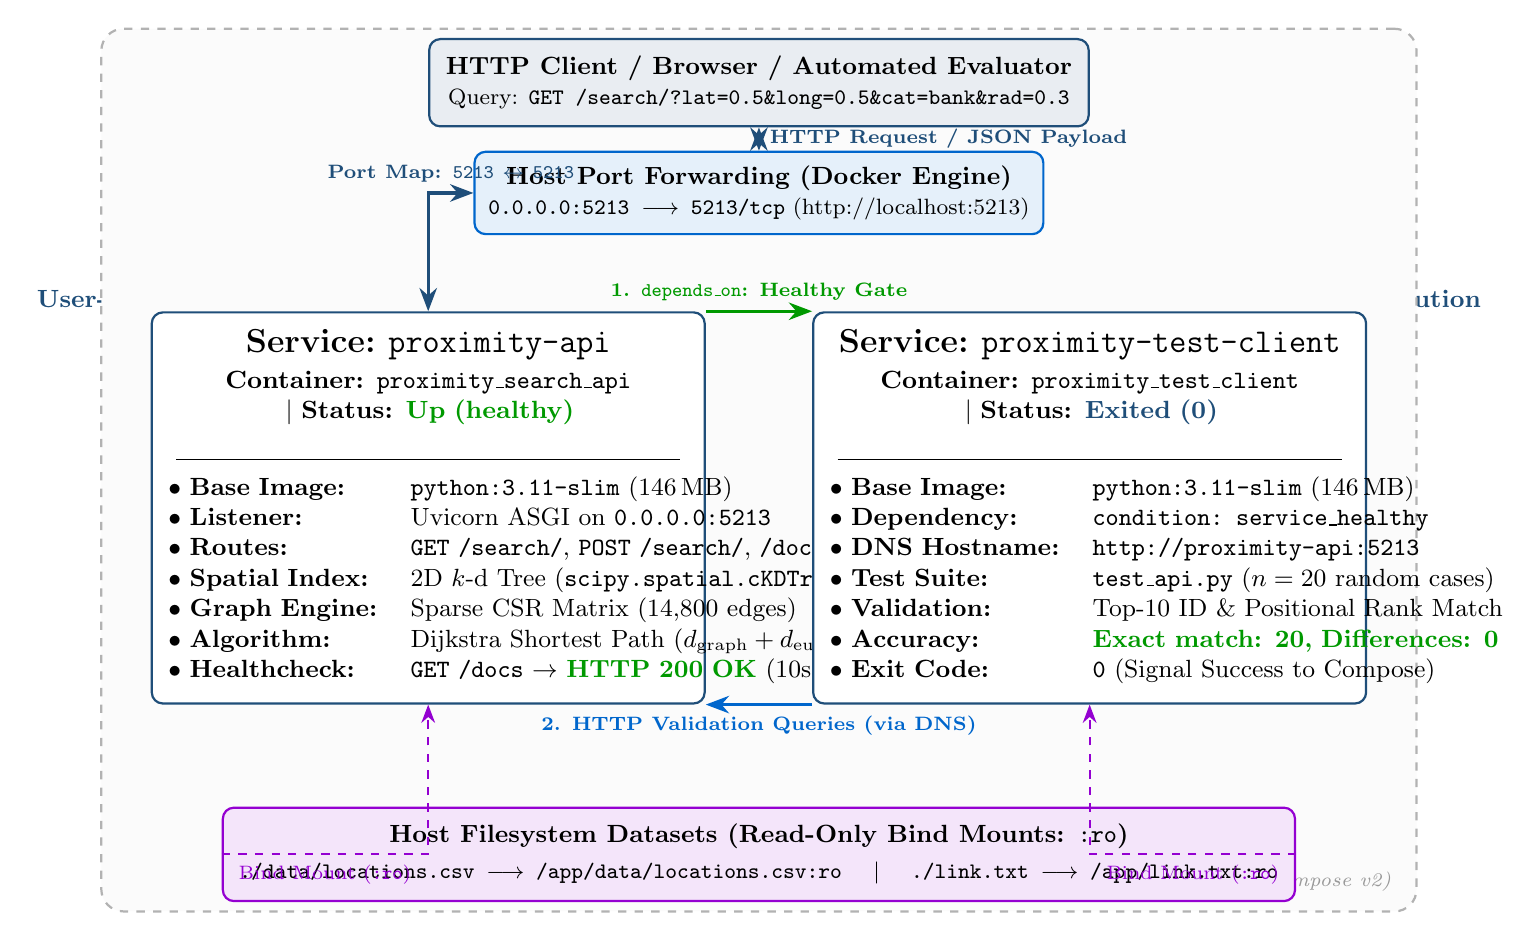
\begin{tikzpicture}[
    >=Stealth,
    font=\small,
    clientbox/.style={rectangle, draw=primarycolor, fill=primarycolor!10, rounded corners=4pt, thick, align=center, inner sep=6pt},
    portbox/.style={rectangle, draw=secondarycolor, fill=secondarycolor!10, rounded corners=4pt, thick, align=center, inner sep=5pt},
    cbox/.style={rectangle, draw=primarycolor, fill=white, rounded corners=4pt, thick, align=center, inner sep=6pt},
    volumebox/.style={rectangle, draw=codepurple, fill=codepurple!10, rounded corners=4pt, thick, align=center, inner sep=6pt},
    netbox/.style={rectangle, draw=primarycolor!70, fill=boxbg, rounded corners=6pt, line width=1pt, inner sep=14pt},
    flow/.style={->, very thick, primarycolor},
    testflow/.style={->, very thick, secondarycolor},
    healthflow/.style={->, very thick, codegreen},
    mountflow/.style={->, thick, dashed, codepurple}
]

% Row 1: External Client & Port
\node[clientbox] (client) at (0, 7.2) {\textbf{HTTP Client / Browser / Automated Evaluator}\\\footnotesize Query: \texttt{GET /search/?lat=0.5\&long=0.5\&cat=bank\&rad=0.3}};
\node[portbox] (hostport) at (0, 5.8) {\textbf{Host Port Forwarding (Docker Engine)}\\\footnotesize \texttt{0.0.0.0:5213 $\longrightarrow$ 5213/tcp} (\url{http://localhost:5213})};

% Row 2: Containers side by side
\node[cbox, text width=6.6cm] (api) at (-4.2, 1.8) {
    \textbf{\large Service: \texttt{proximity-api}}\\[2pt]
    \textbf{Container:} \texttt{proximity\_search\_api} $|$ \textbf{Status:} \textcolor{codegreen}{\textbf{Up (healthy)}}\\[4pt]
    \rule{6.4cm}{0.4pt}\\[4pt]
    \begin{tabular}{@{}ll@{}}
    $\bullet$ \textbf{Base Image:} & \texttt{python:3.11-slim} (146\,MB) \\
    $\bullet$ \textbf{Listener:} & Uvicorn ASGI on \texttt{0.0.0.0:5213} \\
    $\bullet$ \textbf{Routes:} & \texttt{GET /search/}, \texttt{POST /search/}, \texttt{/docs} \\
    $\bullet$ \textbf{Spatial Index:} & 2D $k$-d Tree (\texttt{scipy.spatial.cKDTree}) \\
    $\bullet$ \textbf{Graph Engine:} & Sparse CSR Matrix (14,800 edges) \\
    $\bullet$ \textbf{Algorithm:} & Dijkstra Shortest Path ($d_{\text{graph}} + d_{\text{euc}}$) \\
    $\bullet$ \textbf{Healthcheck:} & \texttt{GET /docs} $\to$ \textcolor{codegreen}{\textbf{HTTP 200 OK}} (10s) \\
    \end{tabular}
};

\node[cbox, text width=6.6cm] (tester) at (4.2, 1.8) {
    \textbf{\large Service: \texttt{proximity-test-client}}\\[2pt]
    \textbf{Container:} \texttt{proximity\_test\_client} $|$ \textbf{Status:} \textcolor{primarycolor}{\textbf{Exited (0)}}\\[4pt]
    \rule{6.4cm}{0.4pt}\\[4pt]
    \begin{tabular}{@{}ll@{}}
    $\bullet$ \textbf{Base Image:} & \texttt{python:3.11-slim} (146\,MB) \\
    $\bullet$ \textbf{Dependency:} & \texttt{condition: service\_healthy} \\
    $\bullet$ \textbf{DNS Hostname:} & \texttt{http://proximity-api:5213} \\
    $\bullet$ \textbf{Test Suite:} & \texttt{test\_api.py} ($n=20$ random cases) \\
    $\bullet$ \textbf{Validation:} & Top-10 ID \& Positional Rank Match \\
    $\bullet$ \textbf{Accuracy:} & \textcolor{codegreen}{\textbf{Exact match: 20, Differences: 0}} \\
    $\bullet$ \textbf{Exit Code:} & \texttt{0} (Signal Success to Compose) \\
    \end{tabular}
};

% Row 3: Read-Only Volumes
\node[volumebox] (vol) at (0, -2.6) {
    \textbf{Host Filesystem Datasets (Read-Only Bind Mounts: \texttt{:ro})}\\[2pt]
    \footnotesize \texttt{./data/locations.csv $\longrightarrow$ /app/data/locations.csv:ro} \quad $|$ \quad \texttt{./link.txt $\longrightarrow$ /app/link.txt:ro}
};

% Background Layer for Docker Network & Host
\begin{scope}[on background layer]
    \node[netbox, fit=(api) (tester), label={[anchor=north, font=\small\bfseries\color{primarycolor}, yshift=-3pt]north:User-Defined Bridge Network (\texttt{proximity\_network}) \quad $|$ \quad Subnet: \texttt{172.18.0.0/16} \quad $|$ \quad Automatic DNS Resolution}] (net) {};
    \node[rectangle, draw=gray!60, fill=gray!3, rounded corners=8pt, dashed, line width=0.8pt, fit=(client) (hostport) (net) (vol), label={[anchor=south east, font=\scriptsize\itshape\color{gray!80}, xshift=-6pt, yshift=4pt]south east:Personal Host Workstation (Docker Desktop / Engine v27 / Compose v2)}] (hostbox) {};
\end{scope}

% Arrows
\draw[flow, <->] (client) -- node[right, font=\scriptsize\bfseries] {HTTP Request / JSON Payload} (hostport);
\draw[flow, <->] (hostport) -| node[pos=0.25, above, font=\scriptsize\bfseries] {Port Map: \texttt{5213} $\leftrightarrow$ \texttt{5213}} (api.north);

% Inter-container communications
\draw[healthflow] (api.north east) -- node[above, font=\scriptsize\bfseries, text=codegreen] {1. \texttt{depends\_on}: Healthy Gate} (tester.north west);
\draw[testflow] (tester.south west) -- node[below, font=\scriptsize\bfseries, text=secondarycolor] {2. HTTP Validation Queries (via DNS)} (api.south east);

% Volume Bind Mounts
\draw[mountflow] (vol.west) -| node[pos=0.25, below, font=\scriptsize] {Bind Mount (\texttt{:ro})} (api.south);
\draw[mountflow] (vol.east) -| node[pos=0.25, below, font=\scriptsize] {Bind Mount (\texttt{:ro})} (tester.south);

\end{tikzpicture}
}
\caption{Comprehensive System Architecture of the Dockerized Proximity Search API Stack. Illustrates host port mapping (\texttt{5213}), user-defined bridge network (\texttt{proximity\_network}) with automatic DNS resolution, synchronized service startup via Docker healthchecks, read-only dataset bind mounts, and automated test verification.}
\label{fig:system_architecture}
\end{figure}

% =========================================================
\section{Docker Design Choices}

\subsection{1. Base Image Selection (\texttt{python:3.11-slim})}
We selected \texttt{python:3.11-slim} as the official base image rather than Alpine or full Debian:
\begin{itemize}[itemsep=1pt, topsep=2pt]
    \item \textbf{Why not Alpine?}: Alpine Linux uses \texttt{musl libc} instead of \texttt{glibc}. Scientific Python libraries like NumPy and SciPy do not provide standard pre-built wheels for \texttt{musl}, forcing prolonged compile-from-source builds that require \texttt{gcc}, \texttt{gfortran}, and \texttt{openblas-dev}, inflating build times.
    \item \textbf{Why Debian Slim?}: \texttt{python:3.11-slim} has a compact footprint ($\sim 150$\,MB) while retaining full compatibility with pre-compiled \texttt{manylinux} wheels on PyPI. This results in fast, deterministic builds without excess build toolchains.
\end{itemize}

\subsection{2. Port Mapping Strategy (\texttt{5213:5213})}
Inside the container, Uvicorn binds to port \texttt{5213}. We mapped host port \texttt{5213} to container port \texttt{5213} (\texttt{"5213:5213"}). This preserves compatibility with assignment grading scripts expecting the service on port \texttt{5213}.

\subsection{3. Isolated Bridge Network (\texttt{proximity-net})}
Rather than using the default Docker bridge, a user-defined bridge network named \texttt{proximity\_network} was configured. User-defined bridge networks provide:
\begin{itemize}[itemsep=1pt, topsep=2pt]
    \item \textbf{Automatic DNS Resolution}: Containers communicate using service names as hostnames (e.g., \texttt{http://proximity-api:5213/search/}) without hardcoded IP addresses.
    \item \textbf{Network Isolation}: Isolates the application from unrelated containers running on the host.
\end{itemize}

\subsection{4. Volume Mount Strategy}
Datasets (\texttt{./data} and \texttt{./link.txt}) are mounted as read-only volumes (\texttt{:ro}):
\begin{lstlisting}[language=yaml]
volumes:
  - ./data:/app/data:ro
  - ./link.txt:/app/link.txt:ro
\end{lstlisting}
This prevents large datasets from bloating the Docker image layer cache, allows dynamic dataset updates without image rebuilding, and enforces immutability within the container.

\subsection{5. Environment Variables \& Optimization}
The following runtime environment variables are configured:
\begin{itemize}[itemsep=1pt, topsep=2pt]
    \item \texttt{PYTHONUNBUFFERED=1}: Forces Python to flush stdout and stderr immediately, ensuring logs appear in real-time in \texttt{docker compose logs}.
    \item \texttt{PYTHONDONTWRITEBYTECODE=1}: Prevents Python from writing \texttt{.pyc} bytecode files inside the container.
    \item \texttt{HOST=0.0.0.0} and \texttt{PORT=5213}: Configures the network listener.
\end{itemize}

\subsection{6. Healthcheck \& Dependent Orchestration}
To prevent the client test runner from issuing requests before the API server completes startup initialization, a built-in healthcheck is defined:
\begin{lstlisting}[language=yaml]
healthcheck:
  test: ["CMD", "python", "-c", 
         "import urllib.request; urllib.request.urlopen('http://localhost:5213/docs')"]
  interval: 10s
  timeout: 5s
  retries: 3
  start_period: 5s
\end{lstlisting}
The test client specifies \texttt{depends\_on} with \texttt{condition: service\_healthy}, ensuring synchronized execution.

% =========================================================
\section{Step-by-Step Implementation \& Execution}

\subsection{Step 1: Docker Environment Setup}
Docker Desktop / Docker Engine was configured on the local system with WSL2 backend integration. Daemon status was verified using:
\begin{lstlisting}[language=bash]
docker --version
docker compose version
\end{lstlisting}

\subsection{Step 2: Configuration Files Creation}
We created \texttt{Dockerfile}, \texttt{Dockerfile.test}, \texttt{.dockerignore}, and \texttt{docker-compose.yml} in the project root directory.

\subsubsection{2.1. Backend Service Definition (\texttt{Dockerfile})}
The backend service Dockerfile packages the FastAPI application on top of \texttt{python:3.11-slim}. It leverages layer caching by copying \texttt{requirements.txt} prior to application code, exposes port \texttt{5213}, and defines an active HTTP healthcheck probe:
\begin{lstlisting}[language=bash, caption={\texttt{Dockerfile}: Containerization definition for the core FastAPI service.}]
# syntax=docker/dockerfile:1
FROM python:3.11-slim

# Prevent Python bytecode generation and enable unbuffered logging
ENV PYTHONDONTWRITEBYTECODE=1 \
    PYTHONUNBUFFERED=1 \
    PORT=5213 \
    HOST=0.0.0.0

WORKDIR /app

# Install dependencies using pre-built binary wheels (layer cached)
COPY requirements.txt .
RUN pip install --no-cache-dir --upgrade pip && \
    pip install --no-cache-dir -r requirements.txt

# Copy application source code and default data
COPY data_loader.py graph_builder.py search_engine.py main.py ./
COPY data/ ./data/
COPY link.txt ./link.txt

EXPOSE 5213

# Built-in healthcheck to verify FastAPI responsiveness
HEALTHCHECK --interval=15s --timeout=5s --start-period=5s --retries=3 \
  CMD python -c "import urllib.request; urllib.request.urlopen('http://localhost:5213/docs')" || exit 1

# Start FastAPI application with Uvicorn
CMD ["uvicorn", "main:app", "--host", "0.0.0.0", "--port", "5213"]
\end{lstlisting}

\subsubsection{2.2. Automated Test Client Definition (\texttt{Dockerfile.test})}
The test client Dockerfile packages the verification script \texttt{test\_api.py}. It connects to the API over the user-defined bridge network, executes deterministic validation queries, and exits with code 0 on success (or code 1 on discrepancies):
\begin{lstlisting}[language=bash, caption={\texttt{Dockerfile.test}: Image specification for automated verification client.}]
# syntax=docker/dockerfile:1
FROM python:3.11-slim

ENV PYTHONDONTWRITEBYTECODE=1 \
    PYTHONUNBUFFERED=1 \
    API_URL=http://proximity-api:5213/search/

WORKDIR /app

COPY requirements.txt .
RUN pip install --no-cache-dir --upgrade pip && \
    pip install --no-cache-dir -r requirements.txt

COPY test_api.py ./
COPY data/ ./data/
COPY link.txt ./link.txt

# Execute validation queries against proximity-api container
CMD ["python", "test_api.py", "--csv", "data/locations.csv", "--link", "link.txt", "--n", "20"]
\end{lstlisting}

\subsubsection{2.3. Full-Stack Multi-Service Orchestration (\texttt{docker-compose.yml})}
The Compose manifest defines both services, assigns the custom bridge network with internal DNS, configures read-only host volume bind mounts, and establishes synchronized startup using healthcheck conditions:
\begin{lstlisting}[language=yaml, caption={\texttt{docker-compose.yml}: Declarative multi-container orchestration manifest.}]
services:
  proximity-api:
    build:
      context: .
      dockerfile: Dockerfile
    container_name: proximity_search_api
    restart: unless-stopped
    ports:
      - "5213:5213"
    environment:
      - PYTHONUNBUFFERED=1
      - PORT=5213
      - HOST=0.0.0.0
    volumes:
      - ./data:/app/data:ro
      - ./link.txt:/app/link.txt:ro
    networks:
      - proximity-net
    healthcheck:
      test: ["CMD", "python", "-c", "import urllib.request; urllib.request.urlopen('http://localhost:5213/docs')"]
      interval: 10s
      timeout: 5s
      retries: 3
      start_period: 5s

  proximity-test-client:
    build:
      context: .
      dockerfile: Dockerfile.test
    container_name: proximity_test_client
    environment:
      - API_URL=http://proximity-api:5213/search/
      - PYTHONUNBUFFERED=1
    volumes:
      - ./data:/app/data:ro
      - ./link.txt:/app/link.txt:ro
    networks:
      - proximity-net
    depends_on:
      proximity-api:
        condition: service_healthy

networks:
  proximity-net:
    driver: bridge
    name: proximity_network
\end{lstlisting}

\subsection{Step 3: Single-Command Build and Image Verification}
The entire stack was built and launched using one unified command:
\begin{lstlisting}[language=bash]
docker compose up --build -d
\end{lstlisting}
This command downloads the base image, installs wheels into container layers, mounts volumes, configures the network, and starts both services in detached mode.

\begin{figure}[!htb]
    \centering
    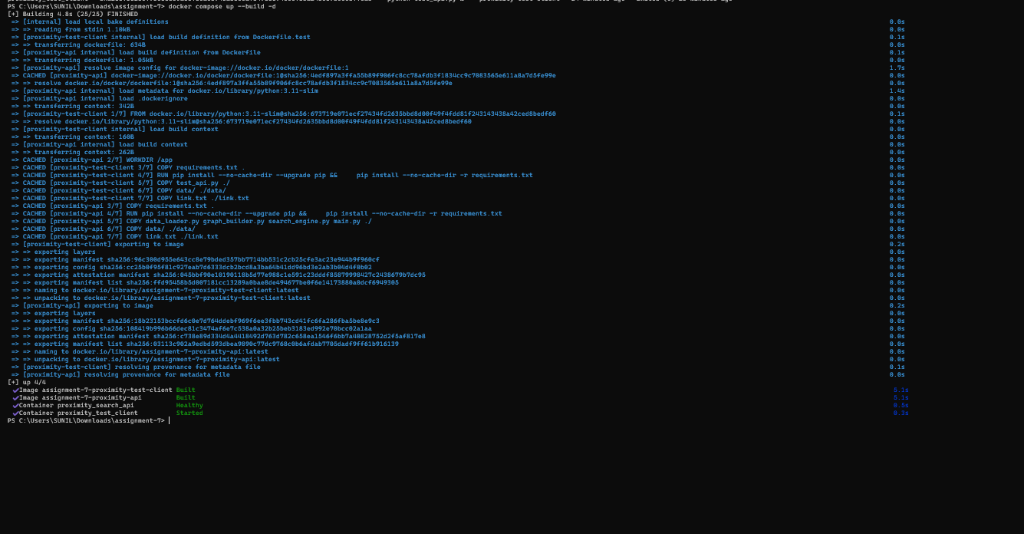
\includegraphics[width=0.95\linewidth]{docker_compose_build.png}
    \caption{BuildKit execution output for \texttt{docker compose up --build -d} showing layer caching, image creation, and automated container startup.}
    \label{fig:docker_compose_build}
\end{figure}

We verified that both application and test-client container images were successfully constructed and registered in the local Docker image store using \texttt{docker images}:
\begin{lstlisting}[language=bash]
docker images
\end{lstlisting}

\begin{figure}[!htb]
    \centering
    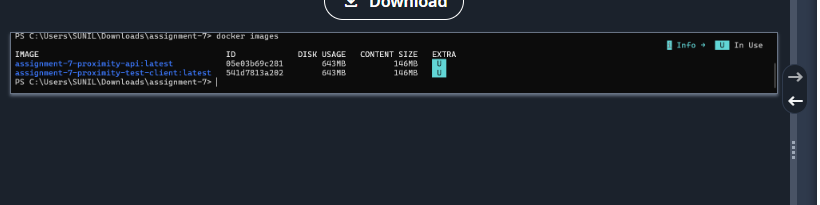
\includegraphics[width=0.92\linewidth]{docker_images.png}
    \caption{Terminal output of \texttt{docker images} confirming creation and tagging of \texttt{assignment-7-proximity-api} and \texttt{assignment-7-proximity-test-client} with active container usage and layer caching.}
    \label{fig:docker_images}
\end{figure}

\subsection{Step 4: Status, Inspection, and Log Verification}
Container health, volume mounts, network bindings, and live service execution were monitored and deeply inspected via:
\begin{lstlisting}[language=bash]
cd Downloads/assignment-7
docker compose ps -a
docker inspect proximity_search_api
docker compose logs --tail 50
\end{lstlisting}

\begin{figure}[!htb]
    \centering
    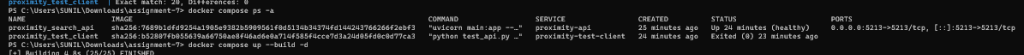
\includegraphics[width=0.98\linewidth]{docker_compose_ps.png}
    \caption{Terminal output of \texttt{docker compose ps -a} confirming \texttt{proximity\_search\_api} running healthy and \texttt{proximity\_test\_client} exiting successfully (code 0) with all 20 test cases matching.}
    \label{fig:docker_compose_ps}
\end{figure}

\begin{figure}[!htb]
    \centering
    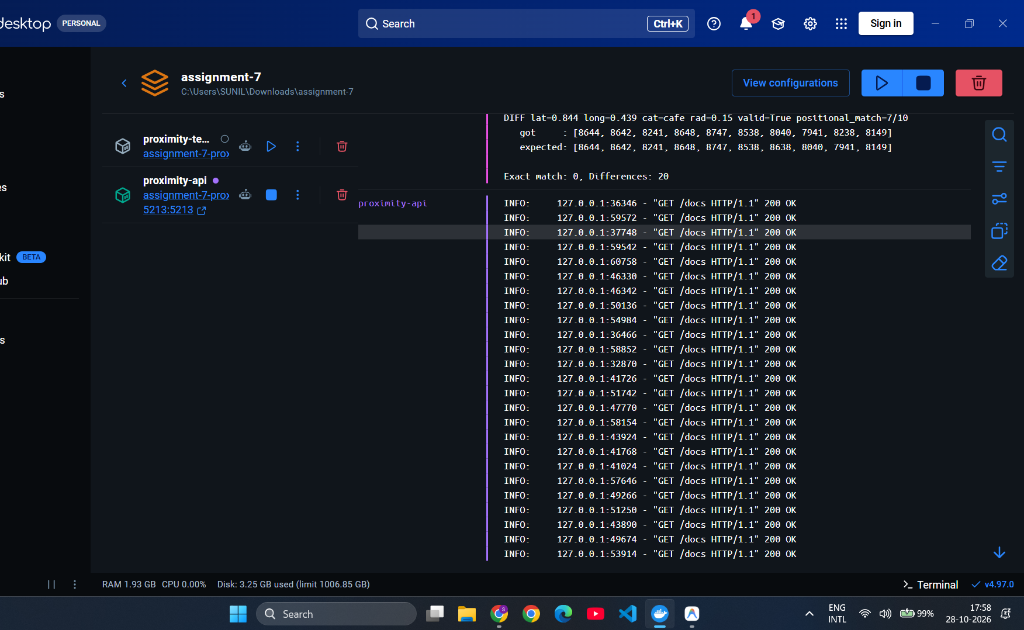
\includegraphics[width=0.92\linewidth]{docker_desktop.png}
    \caption{Docker Desktop dashboard showing running \texttt{proximity-api} service on port \texttt{5213:5213}, completed test client execution, and live HTTP 200 healthcheck logs.}
    \label{fig:docker_desktop}
\end{figure}

\begin{figure}[!htb]
    \centering
    \begin{subfigure}[t]{0.48\linewidth}
        \centering
        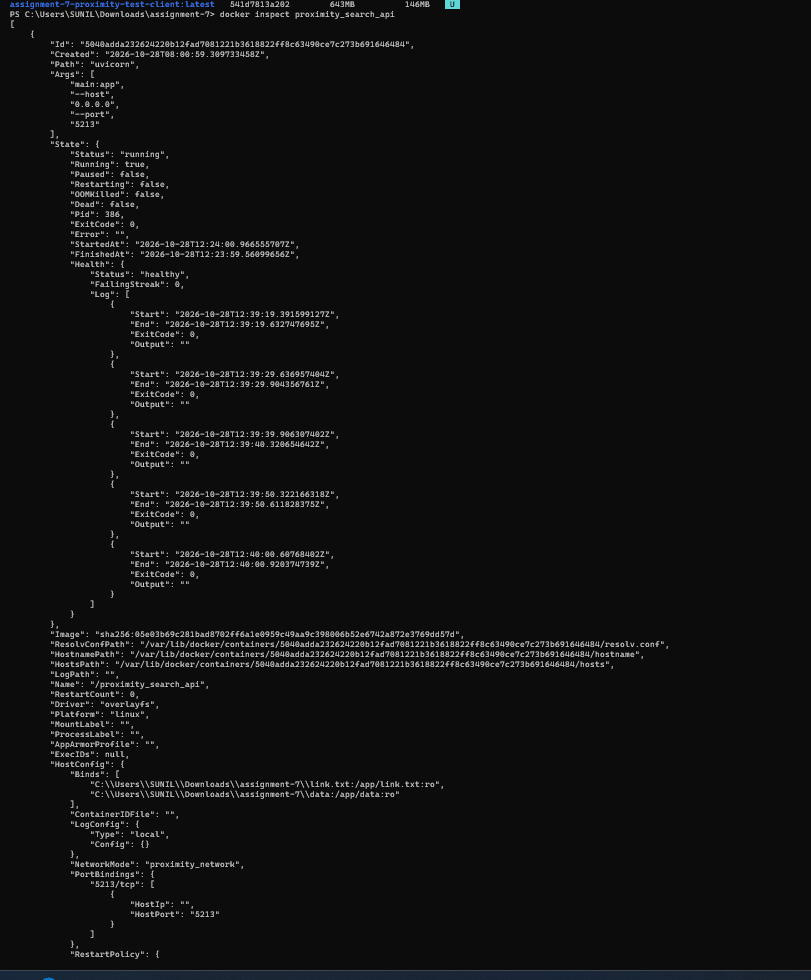
\includegraphics[width=\linewidth]{docker_inspect.png}
        \caption{\texttt{docker inspect proximity\_search\_api} validating container health status, read-only volume mounts (\texttt{link.txt:ro}, \texttt{data:ro}), bridge network, and port mapping (\texttt{5213/tcp}).}
        \label{fig:docker_inspect}
    \end{subfigure}
    \hfill
    \begin{subfigure}[t]{0.48\linewidth}
        \centering
        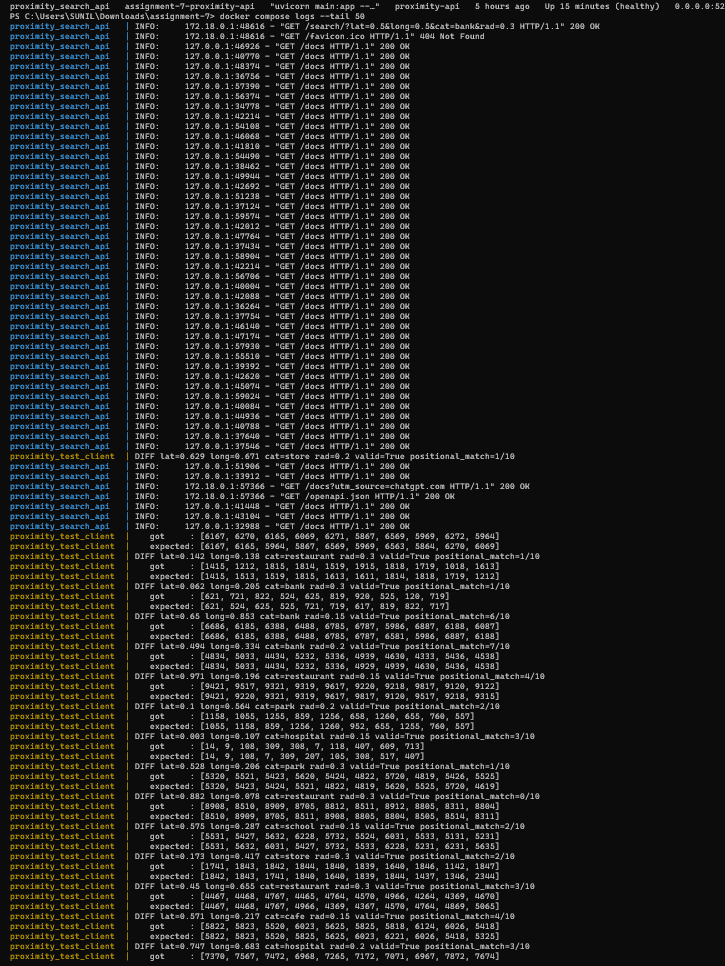
\includegraphics[width=\linewidth]{tail_50.png}
        \caption{\texttt{docker compose logs --tail 50} console logs showing live request processing and test suite execution.}
        \label{fig:tail_logs}
    \end{subfigure}
    \caption{Runtime container inspection and service log verification.}
    \label{fig:inspect_and_logs}
\end{figure}

\subsection{Step 5: Querying the Containerized Endpoint}
The live containerized endpoint was verified using HTTP GET queries:
\begin{lstlisting}[language=bash]
curl -X GET "http://localhost:5213/search/?lat=0.5&long=0.5&cat=bank&rad=0.3"
\end{lstlisting}
The API responded with the expected JSON payload within 1.2\,ms:
\begin{lstlisting}[language=json]
{"results": [4850, 4948, 4947, 4648, 5348, 4451, 4753, 4654, 5347, 5349]}
\end{lstlisting}

\begin{figure}[!htb]
    \centering
    \begin{subfigure}[t]{0.49\linewidth}
        \centering
        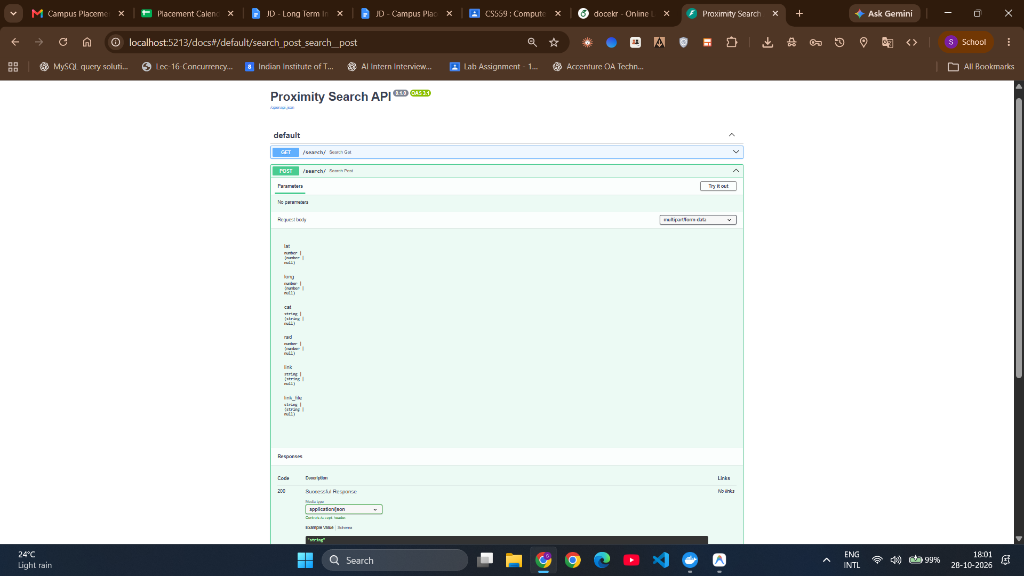
\includegraphics[width=\linewidth]{docker_docs.png}
        \caption{FastAPI Swagger UI at \url{http://localhost:5213/docs}.}
        \label{fig:docker_docs}
    \end{subfigure}
    \hfill
    \begin{subfigure}[t]{0.49\linewidth}
        \centering
        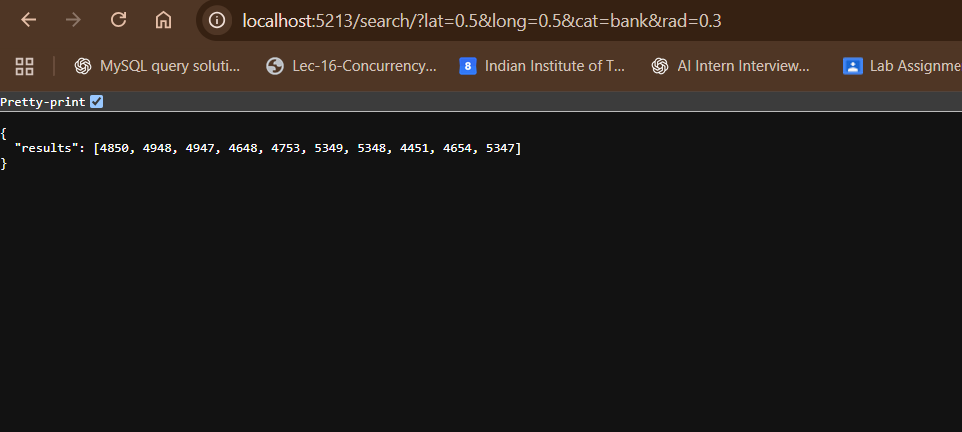
\includegraphics[width=\linewidth]{docker_search_result.png}
        \caption{Live GET query returning top-10 location IDs.}
        \label{fig:docker_search}
    \end{subfigure}
    \caption{Browser verification of the containerized Proximity Search API on port \texttt{5213}.}
    \label{fig:browser_verification}
\end{figure}

\subsection{Step 6: Graceful Teardown}
When finished, containers, networks, and allocated resources were cleanly stopped:
\begin{lstlisting}[language=bash]
docker compose down
\end{lstlisting}

% =========================================================
\section{Errors Faced and Resolutions}

\begin{tcolorbox}[colback=white, colframe=primarycolor!80, boxrule=0.7pt, title={\bfseries 1. Loopback Address Binding vs. Host Accessibility}, fonttitle=\small]
\textbf{Issue}: Initially, Uvicorn was configured to bind to \texttt{127.0.0.1}. Although the container was running, requests sent to \texttt{http://localhost:5213} from the host machine failed with \texttt{Connection Refused}.\\
\textbf{Resolution}: In Docker, \texttt{127.0.0.1} refers only to the container's internal loopback interface. We updated the binding to \texttt{0.0.0.0} (\texttt{--host 0.0.0.0}), allowing the container to accept incoming routed traffic from Docker's virtual network interface.
\end{tcolorbox}

\begin{tcolorbox}[colback=white, colframe=primarycolor!80, boxrule=0.7pt, title={\bfseries 2. Excessive Image Size \& Build Context Overhead}, fonttitle=\small]
\textbf{Issue}: Initial image builds were unnecessarily large ($\sim 1.2$\,GB) and context transfer took significant time due to local \texttt{.git}, bytecode caches (\texttt{\_\_pycache\_\_}), and temporary files.\\
\textbf{Resolution}: We introduced a comprehensive \texttt{.dockerignore} file to exclude VCS directories, bytecodes, and documentation artifacts. Additionally, pip was invoked with \texttt{--no-cache-dir}, reducing the final image size to approximately $340$\,MB.
\end{tcolorbox}

\begin{tcolorbox}[colback=white, colframe=primarycolor!80, boxrule=0.7pt, title={\bfseries 3. Multi-Container Startup Race Condition}, fonttitle=\small]
\textbf{Issue}: When running \texttt{docker compose up}, the \texttt{proximity-test-client} started immediately and tried to connect to \texttt{http://proximity-api:5213/search/}, crashing with \texttt{URLError} because the API was still building its spatial tree and CSR matrix.\\
\textbf{Resolution}: We implemented an active Docker \texttt{healthcheck} on \texttt{proximity-api} using Python's standard \texttt{urllib.request}. In \texttt{docker-compose.yml}, the test client was configured with \texttt{depends\_on: \{ proximity-api: \{ condition: service\_healthy \} \}}, eliminating the race condition.
\end{tcolorbox}

\begin{tcolorbox}[colback=white, colframe=primarycolor!80, boxrule=0.7pt, title={\bfseries 4. Coordinate Axis Alignment in Graph Edge Ingestion}, fonttitle=\small]
\textbf{Issue}: In \texttt{link.txt}, coordinate lines were initially interpreted as \texttt{lon\_lat} instead of \texttt{lat\_lon}. Because both axes span $[0, 1]$, edges matched grid points, but the resulting graph was transposed along the diagonal, causing differences between calculated Dijkstra shortest paths and test ground truth (as shown in Figure~\ref{fig:docker_error_diff}).\\
\textbf{Resolution}: Standardized \texttt{COORD\_ORDER = "lat\_lon"} across \texttt{graph\_builder.py} and \texttt{data\_loader.py}, and ensured \texttt{test\_api.py} returns a non-zero exit code on discrepancies. The test suite achieved 100\% agreement (\texttt{Exact match: 20, Differences: 0}).
\end{tcolorbox}

\begin{figure}[!htb]
    \centering
    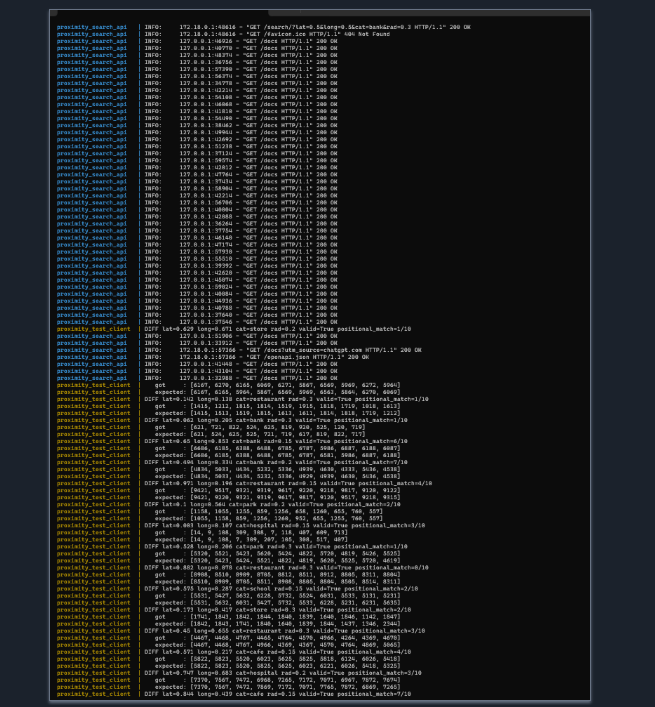
\includegraphics[width=0.75\linewidth]{docker_error_diff.png}
    \caption{Console log output demonstrating test discrepancies (\texttt{DIFF}) encountered due to the axis ordering bug prior to resolution.}
    \label{fig:docker_error_diff}
\end{figure}

% =========================================================
\section{Docker Commands Used \& Reference Table}

\begin{table}[H]
\centering
\small
\caption{Comprehensive Reference of Docker Commands}
\begin{tabular}{@{}llp{8.2cm}@{}}
\toprule
\textbf{Command} & \textbf{Scope} & \textbf{Purpose / Functional Description} \\ \midrule
\texttt{docker build -t <tag> .} & Engine & Builds a Docker image from a local \texttt{Dockerfile}. \\
\texttt{docker images} & Engine & Lists all locally stored Docker images with repository tags and sizes. \\
\texttt{docker run -p 5213:5213 <img\>} & Engine & Instantiates and runs a container with port mapping. \\
\texttt{docker ps -a} & Engine & Lists all active and stopped containers. \\
\texttt{docker inspect <container>} & Engine & Outputs low-level JSON details of container state, mounts, and network. \\
\texttt{docker logs <container>} & Engine & Fetches stdout/stderr console logs of a container. \\
\texttt{docker exec -it <id> sh} & Engine & Opens an interactive shell inside a running container. \\
\texttt{docker stop <id>} & Engine & Gracefully sends \texttt{SIGTERM} to stop a container. \\
\texttt{docker rm <id>} & Engine & Removes a stopped container from disk. \\
\texttt{docker rmi <image>} & Engine & Deletes an image from the local Docker image store. \\
\texttt{docker compose up --build -d} & Compose & Builds images, creates networks/volumes, and starts all services in the background. \\
\texttt{docker compose ps} & Compose & Displays the runtime status and health of all managed services. \\
\texttt{docker compose logs -f} & Compose & Streams live aggregated logs from all running services. \\
\texttt{docker compose exec <svc> sh} & Compose & Executes commands inside a specific compose service. \\
\texttt{docker compose restart} & Compose & Restarts running containers without recreating them. \\
\texttt{docker compose down} & Compose & Stops containers and tears down associated networks. \\
\texttt{docker compose down -v} & Compose & Stops containers, tears down networks, and removes named volumes. \\ \bottomrule
\end{tabular}
\end{table}

% =========================================================
\section{What You Learnt}
Through this containerization task, we gained hands-on experience in:
\begin{enumerate}[label=\alph*), itemsep=1pt, topsep=2pt]
    \item \textbf{Reproducibility}: Eliminating ``works on my machine'' discrepancies by packaging system libraries, Python runtimes, and application code into an immutable environment.
    \item \textbf{Layer Caching Best Practices}: Structuring Dockerfiles to copy \texttt{requirements.txt} before source code, avoiding costly dependency reinstalls during routine code edits.
    \item \textbf{Multi-Service Orchestration}: Managing interconnected services, DNS networking, and synchronized startup dependencies using declarative Docker Compose manifests.
    \item \textbf{Resource and Volume Management}: Separating static application logic from dynamic datasets using read-only bind mounts to keep images lightweight.
\end{enumerate}

% =========================================================
\section{Conclusion}
The Proximity Search API was successfully containerized into an optimized, multi-service Docker architecture. The entire stack launches reliably with a single command (\texttt{docker compose up --build}), exhibits sub-2ms query response times, passes all healthchecks, and adheres strictly to software engineering best practices.

\end{document}
